\begin{figure}
  \centering
    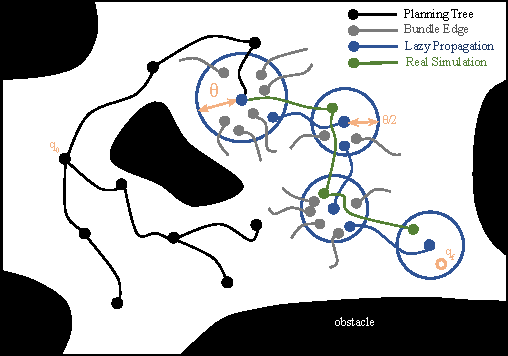
\includegraphics[width=\columnwidth,height=0.7\columnwidth]{assets/theta_over_2.pdf}
  \caption{\textsl{LazyBoE} can lazily propagate a series of edges from $\mathcal{E}$ (shown in \textsl{grey}) in a way that minimizes heuristic cost. After a lazy candidate path is found (\textsl{blue}), a full simulation and collision check is performed along this path (\textsl{green}) to extend the planning tree (\textsl{black}). To ensure the highest rate of success when performing simulation on lazy paths, neighborhood lookup is restricted to $\theta / 2$ for lazy search to allow, in the worst case, the maximum error between the end of a simulated edge and the start of the next lazy edge to be $\theta$.}\label{fig:theta_over_2}
\end{figure}

\subsection{Kinodynamic Motion Planner}\label{sec:methods-planner}
In order to reduce the computational costs associated with dynamics simulation and collision checking, we present a lazy approach for exploring the space of edge bundles $\mathcal{E}$, deferring computation until a viable, low cost approximation to a true candidate path has been found.
Our method, termed \textsl{LazyBoE}, builds upon the design decisions laid out in the BoE planner \cite{shome2021asymptotically}. In addition, it leverages the computed probabilities $P_{\text{lazy\_prop}}$ and $P_{\text{collision}}$ and combines them into the probability of selecting an edge for lazy propagation as $P_{\text{select}} = (1 - P_{\text{collision}}) * P_{\text{lazy\_prop}}$ (\cref{algo:lazyboe}, Line 14). This encourages edges with a lower collision probability to be propagated first, while also promoting lazy propagation. Since the edges are evaluated probabilistically, they can be used more than once, adding diversity and breadth to exploration, countering the downsides of the greedy approach as taken by the BoE planner. Stochasticity thereby avoids local minima and oscillation issues in greedy search.

In the ideal case scenario, all edges can be lazily propagated, enabling us to search through the edge bundle until the goal is reached and doing a real propagation on the shortest path from start to goal. However, this does not hold due to real simulations that may lead to end states beyond the neighborhood radius $\theta < \theta'$ (\cref{fig:pert_analysis}a), thereby resulting in $P_{\text{lazy\_prop}} < 1$ for many edges. Therefore, it becomes important to identify the termination conditions for defining when to stop lazy propagation. These termination conditions (as defined by SHOULD\_TERMINATE\_LAZY() in \cref{algo:lazyboe}, Line 18) are two-fold: i) heuristic value, in our case, the distance to goal state, starts increasing, or; ii) lazy propagation path reaches the goal region $\mathcal{Q}_{goal}$.
As a result, simulation along the lazy path is triggered when these conditions hold, if the preceding edge is not a lazy one, or with probability $1 - P_{\text{select}}$ (\cref{algo:lazyboe}, Line 18).
Next, we demonstrate how these lazy approaches lead to lower planning times and higher success rates in comparison to baseline kinodynamic motion planning algorithms.
